\documentclass{article}
\usepackage[margin=1.25in]{geometry}
\usepackage{amsmath, amssymb, setspace, enumerate, enumitem}
\usepackage{graphicx}
\usepackage[makeroom]{cancel}
\usepackage{datetime}
\usepackage{color,array,graphics}
\usepackage{enumerate}
\usepackage[pdftex, colorlinks, linkcolor=red,citecolor=red,urlcolor=blue]{hyperref}
\usepackage{ulem}

\setlength{\parindent}{0cm}

\setlength{\parskip}{0.3cm plus4mm minus3mm}

\textwidth  6.5in
\oddsidemargin +0.0in
\evensidemargin +0.0in
\textheight 9.0in
\topmargin -0.5in

\usepackage{upquote,textcomp}
\usepackage{amssymb,amsmath,amsfonts,amsthm}
\usepackage{graphicx}
\usepackage{multicol}
\usepackage[T1]{fontenc}
\onehalfspacing

\def\OR{\vee}
\def\AND{\wedge}
\def\imp{\rightarrow}

\DeclareSymbolFont{AMSb}{U}{msb}{m}{n}
\DeclareMathSymbol{\N}{\mathbin}{AMSb}{"4E}
\DeclareMathSymbol{\Z}{\mathbin}{AMSb}{"5A}
\DeclareMathSymbol{\R}{\mathbin}{AMSb}{"52}
\DeclareMathSymbol{\Q}{\mathbin}{AMSb}{"51}
\DeclareMathSymbol{\I}{\mathbin}{AMSb}{"49}
\DeclareMathSymbol{\C}{\mathbin}{AMSb}{"43}

\begin{document}
    \begin{itemize}
        \item \textbf{Problem 7.9.} $G^0 = 0$. $G_1 = 1$ and $G_n = 7G_{n-1} - 12 G_{n-2}$ for $n > 1$. Compute $G_5$. Show $G_n = 4^n - 3^n$ for $n \geq 0$.\\
        \begin{tabular}{ |c|c|c|c|c|c|c| } 
            \hline
            $n$ & 0 & 1 & 2 & 3 & 4 & 5\\ 
            \hline
            $A_n$ & 0 & 1 & 7 & 37 & 175 & 781 \\
            \hline
        \end{tabular}
        \begin{enumerate}[label=(\roman*)]
            \item Prove the base case:
            \begin{align*}
                G(0) = 4^0 - 3^0 = 0
            \end{align*}
            \begin{center}
                base case is true\\
            \end{center}
            \item With induction hypothesis: assume $G(n) = 4^n - 3^n$, prove by direct proof that\\ $G(n) = 4^n - 3^n \rightarrow G(n+1) = 4^{n+1} - 3^{n+1}$ for all $n \geq 0$.
            \begin{align*}
                G(n + 1) &= 7G(n+1-1) - 12G(n+1-2) \text{ (recursive definition)}\\ 
                &= 7G(n) - 12G(n-1)\\
                7G(n) - 12G(n-1) &= 4^{n+1} - 3^{n+1}
            \end{align*}
            \begin{center}
                manipulate the LHS
            \end{center}
            \begin{align*}
                7G(n) - 12G(n-1) &= 7(4^{n} - 3^{n})  - 12(4^{n-1} - 3^{n-1})\text{ (induction hypothesis)}\\
                &= 7(4^n - 3^n) - \cancel{12}(\frac{4^n(3) - 3^n(4)}{\cancel{12}})\\
                &= 7(4^n - 3^n) - (3(4^n) - 4(3^n))\\
                &= 7(4^n) - 7(3^n) - 3(4^n) - 4(3^n)\\
                &= 4(4^n) - 3(3^n)\\
                &= 4^{n+1} - 3^{n+1}
            \end{align*}
            \begin{center}
                We prove the statement is true for $n \geq 0$ by direct proof $\hfill\blacksquare$
            \end{center}

        \end{enumerate}
        \item \textbf{Problem 7.12(c). (See Problem 7.28 for hints.)} Tinker to guess a formula for each recurrence and prove it. In each case $A_1 = 1$ and for $n > 1$:
        \begin{enumerate}[label=(c)]
            \item $A_n = 10nA_{n-1} / (n-1) + n$
            \newline
            \begin{tabular}{ |c|c|c|c|c| } 
                \hline
                $n$ & 2 & 3 & 4 & 5\\ 
                \hline
                $A_n$ & 22 & 333 & 4444 & 55555 \\
                \hline
            \end{tabular}
            \begin{enumerate}[label=\roman*.]
                \item formula found:
                \begin{align*}
                    \frac{10^n-1}{9}n
                \end{align*}
                \item prove the base case:
                \begin{align*}
                    A(2) &= \frac{100-1}{9}(2)\\
                         &= \frac{99}{9}(2) = 22
                \end{align*}
                \begin{center}
                    base case proven
                \end{center}
                \item With induction hypothesis: assume $A(n) = \frac{10^n - 1}{9}n$, prove by direct proof that $A(n) = \frac{10^n - 1}{9}n \rightarrow A(n+1) = \frac{10^{n+1} - 1}{9}(n+1)$ for all $n > 0$.
                \begin{align*}
                    A(n) &= \frac{10nA(n-1)}{n-1}+n\\
                    A(n+1) &= \frac{10(n+1)A(n)}{n} + (n+1) \text{ (recursive definition)}
                \end{align*}
                \begin{center}
                    with with RHS
                \end{center}
                \begin{align*}
                    A(n+1) &= \frac{10(n+1)A(n)}{n} + (n+1) \text{ (induction hypothesis)}\\
                    &= \frac{10(n+1)(\frac{10^n-1}{9}\cancel{n})}{\cancel{n}} + (n+1)\\
                    &= \frac{10(n+1)(10^n-1)}{9} + (n+1)\\
                    &= \frac{(10n+10)(10^n-1) + 9(n+1)}{9}\\
                    &= \frac{10n(10^n) - 10n + 10(10^n) - 10 + 9n + 9}{9}\\
                    &= \frac{10n(10^n) - n + 10^{n+1} - 1}{9}\\
                    &= \frac{10^{n+1}n - n + 10^{n+1} - 1}{9}\\
                    &= \frac{10^{n+1} - 1}{9}(n+1)
                \end{align*}
                \item we prove by direct proof that the statement is true for all $n > 1$ $\hfill \blacksquare$
            \end{enumerate}
        \end{enumerate}
        \item \textbf{Problem 7.13(a).} Analyze these very fast growing recursions. [Hint: Take logarithms.]
       Analyze these very fast growing recursions.
	\begin{align*}
	M_1 &= 2 \text{ and } M_n = aM_{n-1}^2 \text{ for n $\ge 1$}\\
	M_2 &=  aM_{2-1}^2 = a(M_1)^2 = a(2)^2 = 4a\\ 
	M_3 &= aM_{3-1}^2 = a(M_2)^2 = a(4a)^2 = a(16a^2) = 16a^3\\
	M_4 &= aM_{4-1}^2 = a(M_3)^2 = a(16a^3)^2 = a(256a^6) = 256a^7\\
	M_n &= 2^{2^{n-1}}a^{2^{n-1}-1}\\
	\end{align*}
	Can we prove our claim P(n) that $M_n = 2^{2^{n-1}}a^{2^{n-1}-1}$ (thereby removing the recursion)?\\
	Proof. We prove by induction that P(n) is \textbf{T} for n $\ge 1$.\\
	Base Case:\\
	P(1) claims $M_1 = 2^{2^{1-1}}a^{2^{1-1}-1} = 2^{2^{0}}a^{2^{0} - 1} = 2^{1}a^{1 -1} = 2(a^0) = 2(1) = 2$ which is \textbf{T} from the recursive definition.\\
	Induction Step: \\ 
	We prove P(n) $\rightarrow$ P(n+1) for all n $\ge$ 1 via direct proof.\\
	Assume $M_n = 2^{2^{n-1}}a^{2^{n-1}-1}$; we must prove that $M_{n+1} = 2^{2^{(n+1)-1}}a^{2^{(n+1)-1}-1} = 2^{2^n}a^{2^{n}-1}$, n $\in \N$.\\
	LHS:
	\begin{align*}
	M_{n+1} = aM_{n+1-1}^2 &= aM_{n}^2 \text{ (from recursive definition)}\\
	&= a(2^{2^{n-1}}a^{2^{n-1}-1})^2 \text{ (from Induction Hypothesis)}\\
	&= a(2^{(\frac{1}{2})(2^n)}a^{(\frac{1}{2})(2^n)-1})^2\\
	&= a(2^{2^n}a^{2^n -2})\\
	&= 2^{2^n}a^{2^n-1} \text{ (after adding exponents of a)}\\ 
	\end{align*}
	By Induction P(n) is \textbf{T} for all n $\ge$ 1. $\hfill\blacksquare$
	

               \item \textbf{Problem 7.19(d).} Recall the Fibonacci numbers: $F_1$, $F_2 = 1$; and, $F_n = F_{n-1} + F_{n-2}$ for $n > 2$
        \begin{enumerate}[label=(d)]
            \item Prove that every third Fibonacci number, $F_{3n}$, is even
            \begin{enumerate}[label=(\roman*)]
                \item We have to prove that $F_{3n} = 2p$, for some $p \in \mathbb{N}$
                \item prove the base case:
                \begin{align*}
                    F_{3n-1} &= F_2 \text{ when $n=1$, } \rightarrow F_2 = 1\\
                    F_{3n-2} &= F_1 \text{ when $n=1$, } \rightarrow F_1 = 1
                \end{align*}
                \item since the fibonacci sequence is a sum of the previous two terms, we can make the following assumptions:
                \begin{center}
                    By the given formula $F_n = F_{n-1} + F_{n-2}$, we can calculate $F_{3n} = F_{3n-1} + F_{3n-2}$\\
                    We know that both $F_{3n-1}$ and $F_{3n-2}$ are sums of even and odd numbers
                \end{center}
                \begin{align*}
                    F_{3n-1} &= 2k + (2j + 1)\\
                             &= 2(k + j) + 1\\
                    F_{3n-2} &= (2w + 1) + 2i\\
                             &= 2(w + i) + 1
                \end{align*}
                \begin{center}
                    plugging back into the original function, we get:
                \end{center}
                \begin{align*}
                    F_{3n} &= [2(k+j) + 1] + [2(w+i) + 1]\\
                           &= 2(k + j) + 2(w+i) + 2\\
                           &= 2(k + j + w + i + 1)
                \end{align*}
                \begin{center}
                    We prove that the statement is true for all $n > 2$ $\hfill\blacksquare$
                \end{center}
            \end{enumerate}
        \end{enumerate}
        \item \textbf{Problem 7.42.} Give pseudocode for a recursive function that computes $3^{2^n}$ on input $n$.
        \begin{verbatim}
		out = recur(n)
		      if (n == 0) out = 3;
		      else out = recur(n-1) * recur(n-1);
	\end{verbatim}
	Proof. We use induction to prove recur(n) =$ 3^{2^n}$, w/ n $\ge \N_0$.\\
	Base Case:\\
	n = 0: recur(0) $\rightarrow$ out = 3, which is equal to $3^{2^0} = 3^1 = 3 \therefore$ making recur(n) = $3^{2^n}$ \textbf{T}.\\
	Induction Step\\
	We prove recur(n) = $ 3^{2^n} \rightarrow$ recur(n+1) = $ 3^{2^{n+1}}$ is T for all n $\in \N_0$ via a direct proof.\\
	Assume recur(n) = $ 3^{2^n}$\\
	LHS:\\
	\begin{align*}
	\text{recur(n+1)} &= \text{recur((n+1) - 1) * recur((n+1) -1) (from recursive definition)}\\ 
	&= \text{recur(n) * recur(n)}\\
	&= 3^{2^n} * 3^{2^n} \text{ (from Induction Hypothesis)}\\ 
	&= 3^{2(2^n)}\\
	&= 3^{2^{n+1}}\\
	\end{align*}
	By induction, we have proven recur(n+1) = $ 3^{2^{n+1}}$ is \textbf{T} for all n $\ge 0$. Thus recur(n) = $ 3^{2^n}$ is \textbf{T} for all n $\ge 0$.$\hfill\blacksquare$\\
b.
\begin{align*}
T_0 &= 2\\
T_1 &= 7\\
T_2 &= 17\\
T_3 &= 37\\ 
T_n &= 2(T_{n-1}) + 3\\
\end{align*}
After tinkering, $T_n = 5(2^n) - 3$\\
Proof.  We use induction induction to prove  $T_n = 5(2^n) - 3$, for all n $\in \N_0$ via a direct proof.\\
Base Case:\\
 $T_0 = 5(2^0) - 3 = 2$, which is \textbf{T} from the recursive definition.\\
 Induction Step:\\
 We prove  $T_n = 5(2^n) - 3 \rightarrow  T_{n+1} = 5(2^{n+1}) - 1$ is T for all n $\in \N_0$ via direct proof.\\
 Assume  $T_n = 5(2^n) - 3$\\
 LHS:\\
 \begin{align*}
  T_{n+1} &= 2(T_{n + 1 - 1}) + 3  \text{ (from recursive definition)}\\
  &= 2(T_n) + 3\\
  &= 2(5(2^n) - 3) + 3 \text{ (from induction hypothesis)}\\
  &= 5(2^1)(2^n) - 6 + 3\\
  &= 5(2^{n+1}) - 3\\
 \end{align*} 
By induction, we have proven $T_{n+1} = 5(2^{n+1}) - 3$ is \textbf{T} for all n $\in \N_0$. Thus,  $T_n = 5(2^n) - 3$ is \textbf{T} for all n $\in \N_0$.$\hfill\blacksquare$\\



      
        \item \textbf{Problem 7.45(c).} Give recursive definitions for the set $S$ in each of the following cases.
        \begin{enumerate}[label=(c)]
            \item $S =$ \{all strings with the same number of 0's and 1's\} (e.g. 0011,0101,100101).
            \begin{enumerate}[label=\arabic*.]
                \item \textbf{[basis]} $\epsilon \in S, 0 \in S, 1 \in S$
                \item \textbf{[constructor(i)]} $\epsilon \in S \rightarrow 0 \bullet x \bullet 0 \in S$;\\
                \textbf{[constructor(ii)]} $\epsilon \in S \rightarrow 1 \bullet x \bullet 1 \in S$.
            \end{enumerate}
        \end{enumerate}
        \item \textbf{Problem 7.49.} There are 5 rooted binary trees (RBT) with 3 nodes. How many have 4 nodes\\
        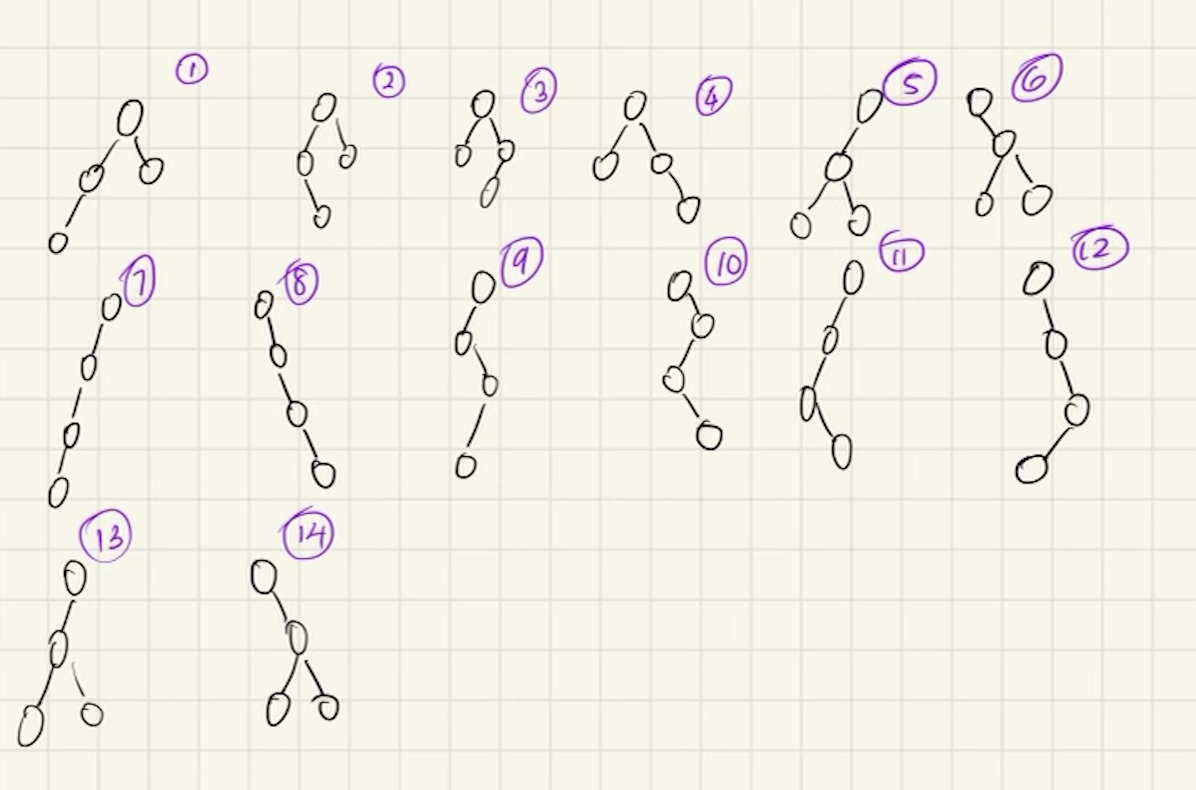
\includegraphics[width=100mm,scale=0.5]{binaryTrees.png}
        \begin{itemize}[label=$\bullet$]
            \item We can make 14 possible rooted binary trees with 4 nodes.
        \end{itemize}
        \item \textbf{Problem 8.12(d).} A set $P$ of parenthesis strings have a recursive definition.
        The strings in P are balanced, i.e. they have an equal number of open and close parentheses. Let us prove it. To do so, imagine creating the strings $s_1,s_2,s_3$,... of P in some order starting w/ $s_1 = \epsilon$\\
        $P = \{\epsilon, [], [[]], [][],....,s_n,....\}$\\
The list has all strings of P in their order of creation. The nth string $s_n$ came from either one previous string $s_i$ or two previous strings $s_i$ and $s_j$ using constructors $s_n = [s_i]$ and $s_n = s_i \times s_j$ respectively. If $s_i$ and $s_j$ are balanced, then so is $s_n$ with one or more open parenthesis and closed parenthesis. Since the primordial ancestor $s_1 = \epsilon$ balanced, we can prove all the strings in P are balanced. \\

Q(n): Every string in P is balanced\\
Proof. We use strong induction to prove Q(n) for n $\ge$ 1\\
Base Case: \\
n = 1: $s_1 = \epsilon$ which is clearly balanced, so Q(1) is true.\\
Induction Step:\\
    We show Q(1)$\wedge$...$\wedge$Q(n) $\rightarrow$ Q(n+1) using direct proof. Assume Q(1),Q(2),...Q(n): 
$s_1$ ,....., $s_n$ are all balanced. We must show Q(n+1): $s_{n+1}$ is balanced. We have that $s_{n_+1} = [s_i]$, where $s_i$ appeared earlier than $s_{n+1}$, so i < n + 1. By the strong induction hypothesis, $s_i$ is balanced so $s_{n+1}$ is balanced because you add one open-parenthesis and close-parenthesis. We also have that $s_{n+1} = s_is_j$ , where $s_i$ and $s_j$ appeared earlier than $s_{n+1}$. By the strong induction hypothesis, $s_i$ and $s_j$ are balanced. Therefore $s_{n+1}$ is balanced because the previous two results used to produce $s_{n+1}$ are balanced.$\hfill\blacksquare$\\


        \item \textbf{Problem 8.14.} A set $A$ is defined recursively as shown.
        \begin{enumerate}[label=\arabic*.]
            \item $3 \in A$.
            \item $x,y \in A \rightarrow x + y \in A$;\\
            $x,y \in A \rightarrow x-y \in A$.
        \end{enumerate}
       $A = \{3, 6, 0,....s_n,....\}$\\
The list has all elements of A in their order of creation. The nth element $s_n$ came from two previous strings $s_i$ and $s_j$ using the constructors $s_n = s_i + s_j$ and $s_n = s_i - s_j$.\\
Q(n): Every element of A is a multiple of 3\\
Base Case: \\
    n = 1 where 1 is the first element in A; $s_1$ = 3 which is a multiple of 3, so Q(1) is true. \\
Induction Step: \\
    We show Q(1)$\wedge$...$\wedge$Q(n) $\rightarrow$ Q(n+1) using direct proof. Assume Q(1), Q(2),...Q(n): $s_1,...s_n$ are all multiples of 3. We must show Q(n+1) is a multiple of 3. We have that $s_{n+1}$ = $s_i$ + $s_j$, so i, j < n+1.  By the strong induction hypothesis, $s_i$ and $s_j$ are both multiples of 3 and come BEFORE $s_{n+1}$. Therefore, $s_{n+1}$ is also a multiple of three because it is the sum (or concatenation) of two multiples of 3. The same can be said about $s_{n+1} = s_i - s_j$, as $s_i$ and $s_j$ are both multiples of three once again, so $s_{n+1}$ is the difference(subtraction) of two multiples of 3, making it itself a multiple of three. By definition, the concatenation/addition and subtraction of multiples of 3 is a multiple of 3. Therefore, $s_{n+1}$ is a multiple of 3 in the case of both constructors.$\hfill\blacksquare$\\


            \item Prove that every multiple of 3 is in $A$.
            \begin{enumerate}[label=\arabic*.]
                \item We prove by contradiction that every multiple of 3 is in $A$. Consider m, a multiple of 3 that is not in $A$.
                \item \textbf{[Case 1]} $k > 0$, $m = 3k$, where $m$ is the largest multiple of 3 NOT in our set $A$.
                \begin{align*}
                    3k = 3 + 3 + 3 + ...
                \end{align*}
                \begin{center}
                    We can consider $3(k+1)$, which we know is in our set since it is larger than $m$
                \end{center}
                \begin{align*}
                    3(k+1) = 3k+3
                \end{align*}
                \begin{center}
                    We know by constructor(ii) that $x-y \in A$, and we know that $3 \in A$ by the basis.
                \end{center}
                \begin{align*}
                    3(k) &= x - y \text{, where } x = 3k + 3 \text{ and } y = 3\\
                         &= 3k + 3 - 3\\
                         &= 3k \text{ woops, we derived a contradiction!}
                \end{align*}
                \item \textbf{[Case 2]} $k < 0$, $m = -3k$, where $m$ is the smallest multiple of 3 NOT in our set A.
                \begin{align*}
                    3(-k) = -3 -3 -3 -3 -3 -3 -...
                \end{align*}
                \begin{center}
                    We can consider $3(-k - 1)$, which we know is in our set since it is smaller than $m$
                \end{center}
                \begin{align*}
                    3(-k-1) = -3k-3
                \end{align*}
                \begin{center}
                    We know by constructor(i) that $x+y \in A$, and we know that $3 \in A$ by the basis.
                \end{center}
                \begin{align*}
                    -3k &= x+y \text{, where } x = -3k -3 \text{ and } y = 3\\
                        &= -3k -3 + 3\\
                        &= -3k \text{ woops, we derived a contradiction!}
                \end{align*}
                \item \textbf{[Case 3]} $k = 0$, $m = 0$, $0$ is not in $A$
                \begin{center}
                    We know from the basis that $x = 3$ and $y = 3$\\
                    From constructor(ii), we can use $x - y$, where:
                \end{center}
                \begin{align*}
                    x - y &\in A\\
                    3 - 3 &\in A\\
                    0 &\in A \text{ woops, we derived a contradiction!}
                \end{align*}
                \item We prove by contradiction for 3 distinct cases of $k$, proving that all multiples of 3 is in $A \hfill\blacksquare$
            \end{enumerate}
    \end{itemize}
    
\end{document}